\documentclass[table]{beamer}
\usetheme{CambridgeUS}
\usepackage[utf8]{inputenc} 
\usepackage{amsmath}
\usepackage[T1]{fontenc}
\usepackage{graphicx}
\usepackage[noend]{algpseudocode}
\usepackage{algorithm}
\usepackage{biblatex}
\usepackage{float}
\usepackage{tikz}
\usepackage[french]{babel}
\usepackage{multirow}


\begin{document}

\title{CYK Probabiliste}  %PAGE 1
\author{Lapraye \& Lévêque \& Viegas}

\institute{Paris VII}
\date{\today}

\addtobeamertemplate{footline}{\insertframenumber/\inserttotalframenumber}

\begin{frame}
 \maketitle
\end{frame}

\begin{frame}
\frametitle{L'Algorithme CYK}
\begin{itemize}% Introduction
% 	but / on se place dans le cadre de l'analyse syntaxique / caractéristiques de l'analyse syntaxique
% 	Ce qu'on veut en entrée du cky / Ce qu'on veut en sortie
% 	Organisation du travail
% 		Etapes d'implémentation
% 			- Extraction
% 			- CYK
% 			- Evaluation et résultats
  \item<1-4>{Un algorithme de parsing ascendant}
  \item<2-4>{Complexité $\mathcal{O}(|G|n^3) $ } %
  \item<3-4>{Parsing tabulaire}
  \item<4-4>{Extention aux grammaire hors-contexte probabilistes (PCFG)}
 \end{itemize}
 
\end{frame}

\begin{frame}
\frametitle{L'Algorithme CYK}
\begin{algorithm}[H]
	\caption{CYK normal}
	\begin{algorithmic}
	\Function{CKY}{$w[1..n]$, $G: < NT, T, P, \rho>$, R[1..n, 1..n]}
			\ForAll {i de 1 à m}
			    \If{$N \rightarrow w_i$}
			      \State{$R[i,i+1]\gets N$ }
			    \EndIf 
			\EndFor
			
			\ForAll{ k de 2 à n}
			    \ForAll{i de 1 à $n-i+2$}
				\ForAll {j de i+1 à i+k}
				      \ForAll{$A \in R[i,j]$}
					    \ForAll{$ $}
						\ForAll{$NT \in P$}
							\If{$NT \rightarrow A B$}
							  \State $R[i,i+k] = R[i,i+k] \cup \{NT\}$
							\EndIf
						\EndFor
					    \EndFor
				      \EndFor
			      \EndFor
			  \EndFor
		      \EndFor
		\If{$S \in R[0,n]$}
		  \Return True
		\EndIf
		\EndFunction
	\end{algorithmic}
\end{algorithm}
\end{frame}


\begin{frame}
 \frametitle{Les PCFG}
 \begin{itemize}
  \item<1-5>{Les CFG : un quadruplet $(\Sigma,V,S,P)$ }
  \item<2-5>{Les CFG pondérées : ajout d'une fonction de poids $ f : p \mapsto \alpha, w \in W, \alpha \in \mathbb{R} $ }
  \item<3-5>{Les CFG probabilistes : les poids correspondent à des probabilités pour une réécriture donnée.  
  $$ f : p \mapsto \alpha, p \in P, \alpha \in [0,1]$$ $$ \forall X \in V, \sum_{X\to\alpha}p(X\to\alpha)=1 $$ }
  \item<4-5>{Les CFG probabilistes représentent un modèle de prédiction déduit à partir du corpus dont elles sont extraites.}
  \item<5-5>{Extraction des PCFG}
 \end{itemize}

\end{frame}



\begin{frame} 
\frametitle{La forme normale de Chomsky (CNF)}
 \begin{itemize}
 \item {l'axiome S est inaccessible}
 \item {Les règles de production adoptent une des formes suivantes, avec  $\varepsilon$ la production vide, $A,B,C,D \in V$, et $e \in \Sigma$ : 
     $$A \rightarrow B C $$ 
     $$ D \rightarrow e $$
     $$ S \rightarrow \varepsilon$$ }

 \end{itemize}

\end{frame}

\begin{frame}
\setbeamercovered{transparent}
 \frametitle{Transformer la grammaire en CNF}
 \begin{enumerate}
 \item<1>{ Faire en sorte que l'axiome n'apparaisse plus dans les parties droites de règles}
 \item<1>{Supprimer les règles d'effacement (c'est à dire de la forme $A \rightarrow^*\varepsilon$ ) pour les non-terminaux autres que l'axiome.}
 \item<1>{Faire en sorte que tout les terminaux apparaissent uniquement dans la partie droite de règles unaires }
 \item<1-2>{Remplacer les règles de production n-aire par des règles binaires équivalentes.}
 \item<1-2>{Supprimer les productions singulières de non-terminaux, c'est à dire les règles de la forme $A \rightarrow B$ avec $A,B \in V$ }
 \end{enumerate}
 
\end{frame}
% 
% \begin{frame}
%  \frametitle{Transformer la grammaire en CNF}
% \end{frame}




% \begin{frame} % PAGE 2
% \frametitle{Plan}
% \tableofcontents
% \end{frame}

\begin{frame}
  \frametitle{Le corpus Sequoia}
  \begin{columns}
  \begin{column}{0.5\textwidth}
    \begin{itemize}
     \item{ Un corpus diversifié}
     \item{ Des phrases de longueur variable}
     \item{ Extraction de la grammaire}
     
     
    \end{itemize}
   
  \end{column}
  
  \begin{column}{0.5\textwidth}
  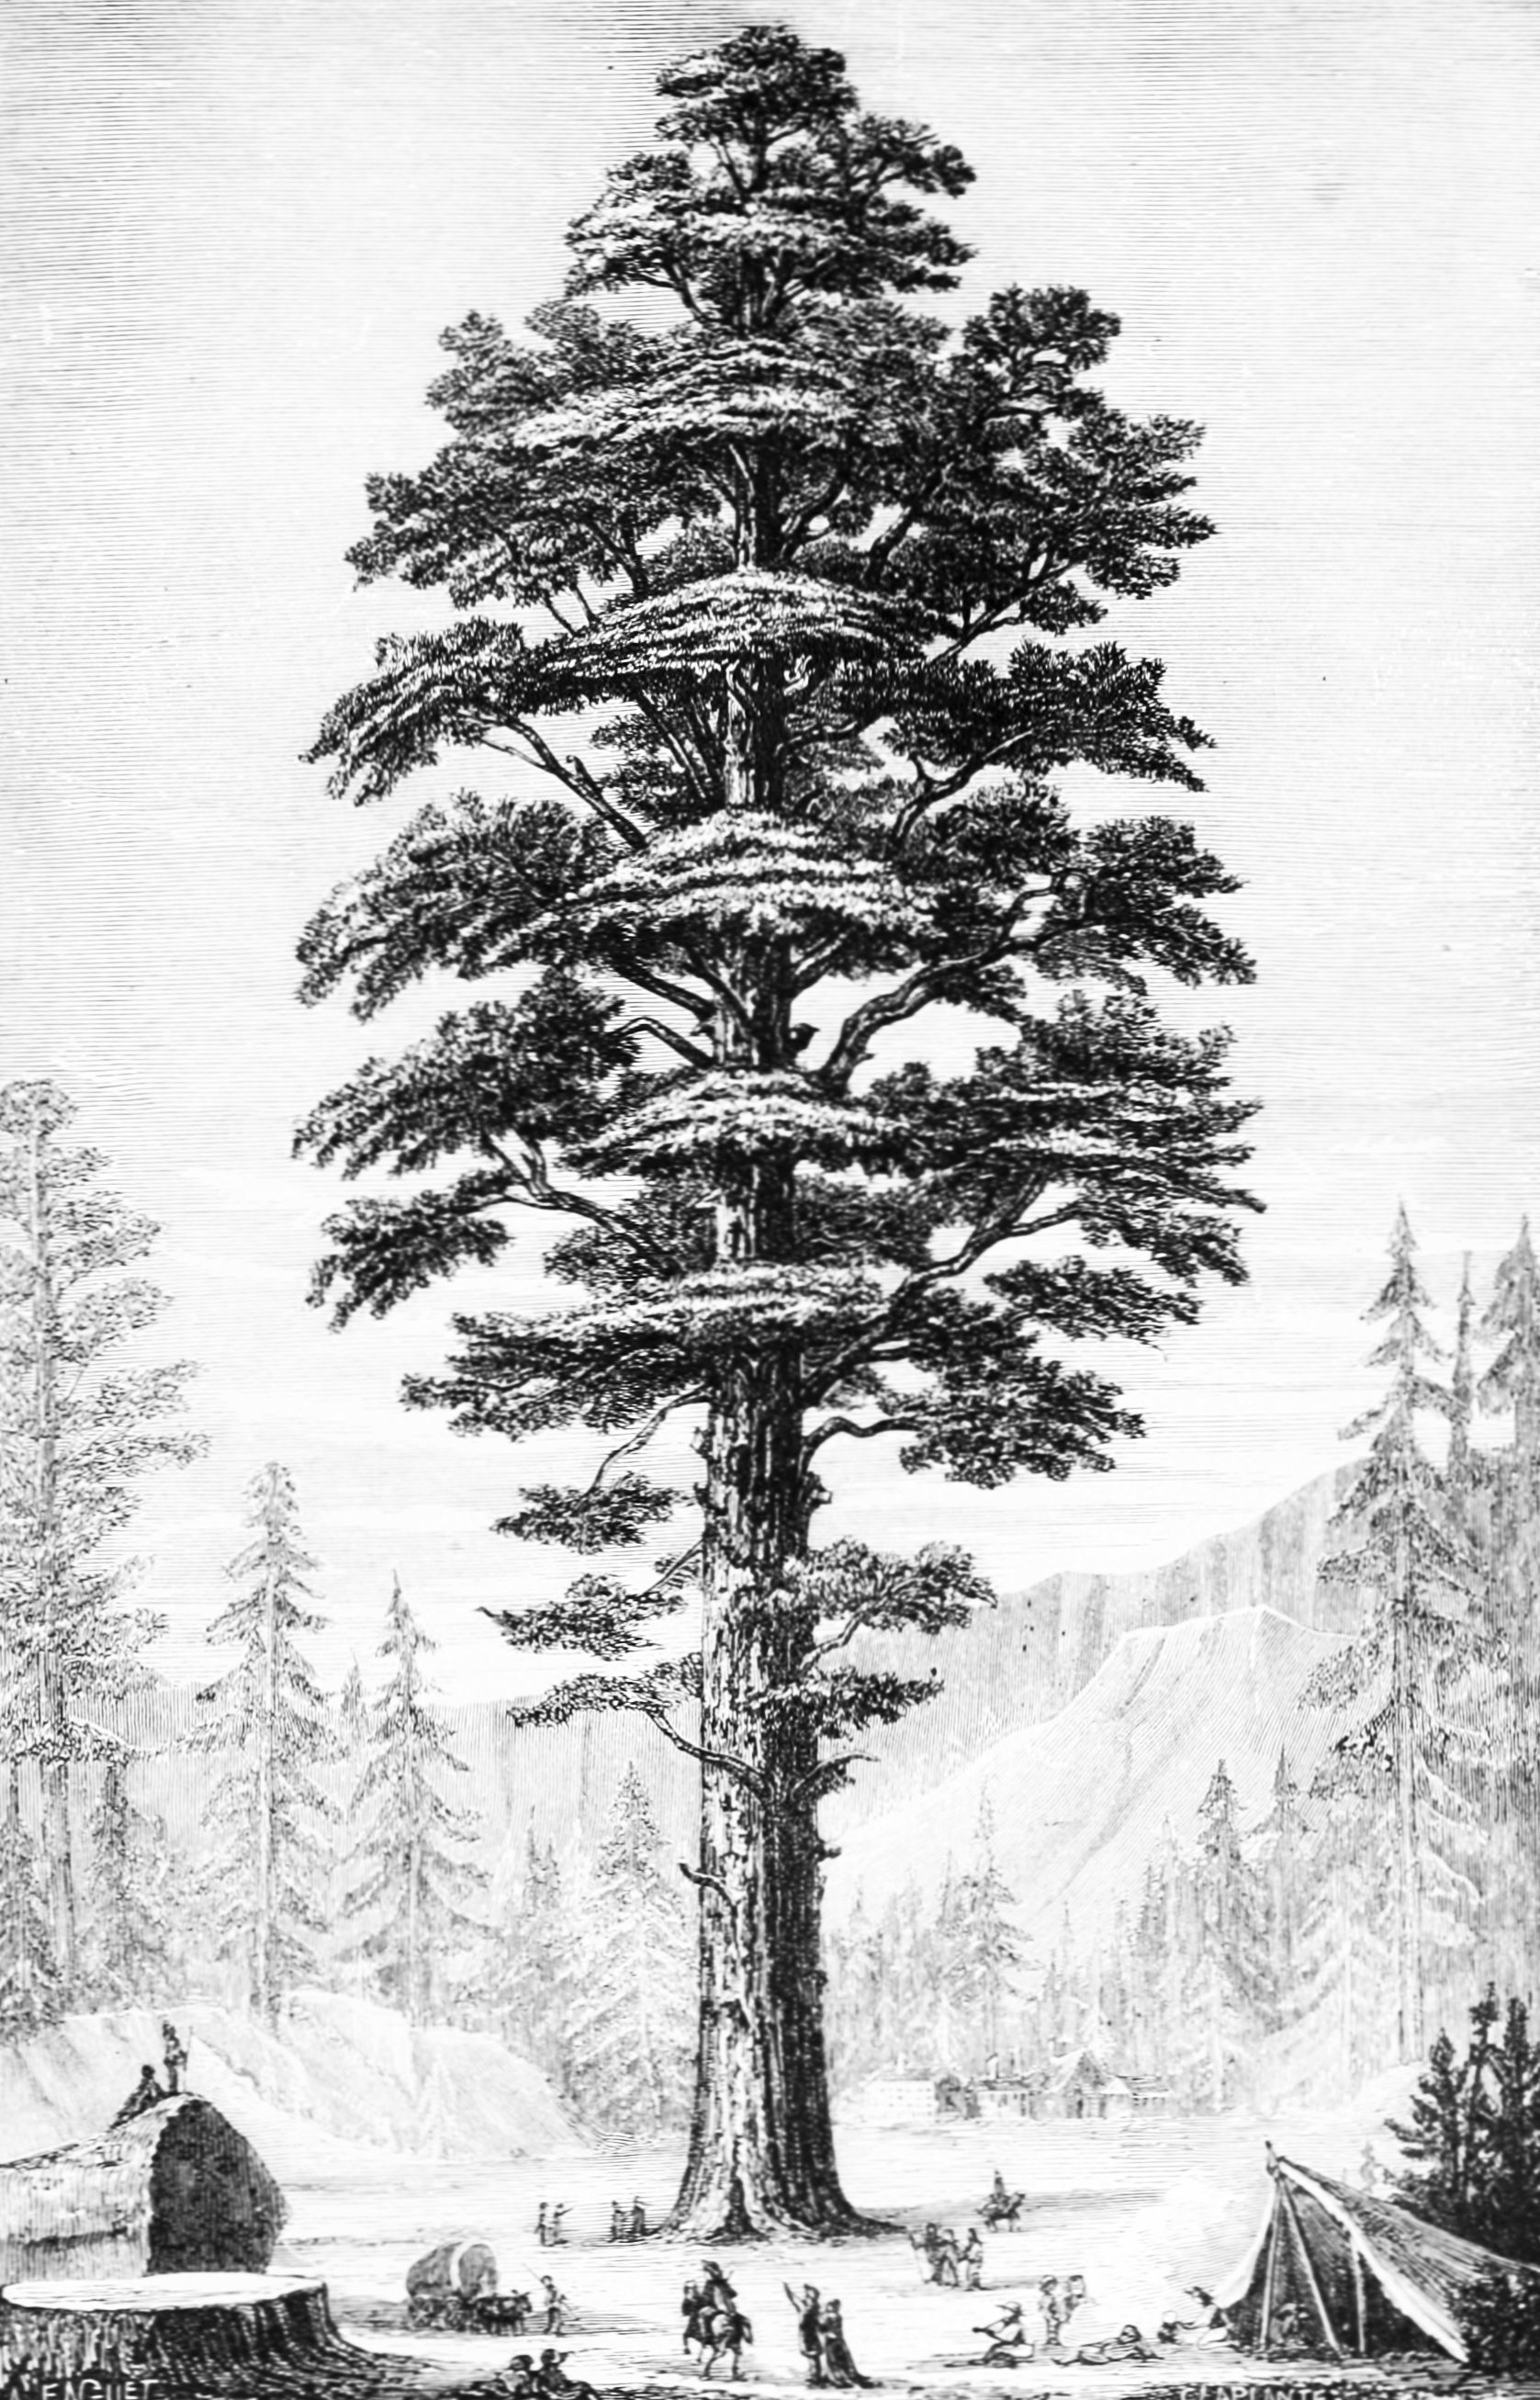
\includegraphics[width=80pt,]{PSM_V03_D341_Sequoia_gigantea_of_california.jpg}  
  \end{column}

  \end{columns}

\end{frame}

\begin{frame}
 \frametitle{L'Algorithme CYK}
	\begin{algorithm}[H]
	\caption{CYK probabiliste (argmax)}
		\small{\begin{algorithmic}
			\Function{CYK}{$w[1..n]$, $G: < NT, T, P, \rho>$, R[1..n, 1..n]} \Comment w : mot; G: Grammaire; C: charte
				\ForAll{$k \gets 2, |n|$} \Comment Boucle \text{gérant} l'empan
					\ForAll{$i \gets k-2, 0$}
						\ForAll{$nt \in NT$} \Comment{Boucle faisant l'argmax }
							\State $best = 0;$
							\ForAll{${nt \rightarrow nt^1 nt^2 \subset P}$}
								\ForAll{$j \gets i+1, k-1$}
									\State $t1 = R[i,j][nt^1]$ 
									\State $t2 = R[j,k][nt^2]$
									\State $candidate = t1 * t2 * \rho(nt \rightarrow nt^1 nt^2  );$
									\If{$candidate > best$}
										\State $best = candidate;$
									\EndIf
								\EndFor
							\EndFor
							\State $R[i,k][nt] = best;$
						\EndFor
					\EndFor
				\EndFor
			\EndFunction
		\end{algorithmic} }
	\end{algorithm}

\end{frame}


\begin{frame}
\frametitle{Notre implémentation du CYK}

\begin{itemize}
 \item<1-3>{Un algorithme gourmand en temps et en mémoire}
 \item<2-3>{Optimiser la recherche des réécritures possibles}
 \item<3>{Le backtracking}
\end{itemize}


 
\end{frame}

\begin{frame}
\frametitle{Evaluation}
\begin{itemize}
 \item<1-3> {Une évaluation problématique.}
 \item<2-3> {La mesure dite de PARSEVAL}
 \item<3> {Précision, Rappel et f-mesure}
\end{itemize}

\end{frame}

\begin{frame}
\frametitle{Résultats}
\begin{center}
\begin{tabular}{|l|r|r|}

    & Étiqueté & Non-étiqueté \\
%    \hline
   Précision & 0.829 & 0.870 \\
%    \hline
   Rappel & 0.828 & 0.868 \\
%    \hline
   F-mesure & 0.829 & 0.869 \\
%    \hline
\end{tabular}


\end{center}

\end{frame}



\begin{frame}
  \frametitle{Références}
  {\footnotesize
  \begin{thebibliography}{1}    
  \beamertemplatebookbibitems
  \bibitem{roark}
    Brian Roark, Richard Sproat.
    \newblock {\em Computational Approaches to Morphology and Syntax}.
    \newblock Oxford University Press, 2007.
  \beamertemplatearticlebibitems
  \bibitem{parserEval}
    Mariana Romanyshyn, Vsevolod Dyomkin.
    \newblock {\em The Dirty Little Secret of Constituency Parser Evaluation}, 2014.
    \newblock {http://tech.grammarly.com/blog/posts/The-Dirty-Little-Secret-of-Constituency-Parser-Evaluation.html}
   \bibitem{LangeLeiss}
    Martin Lange, Hans Leiss
    \newblock{« To CNF or not to CNF : An Efficient Yet Presentable Version of the CYK Algorithm », 2009}
    \newblock{{\em Informatica Didactica} \No 8}
    
    \bibitem{BlackAbney}
     E. Black, S.Abney et al. 
    \newblock{« Procedure for Quantitatively Comparing the Syntactic Coverage of English Grammars »}
    \newblock{1991, DARPA Speech and Natural Language Workshop}
  
  \end{thebibliography}
  }

  %   ¯\_(ツ)_/¯

\end{frame}


\end{document}
